% Options for packages loaded elsewhere
\PassOptionsToPackage{unicode}{hyperref}
\PassOptionsToPackage{hyphens}{url}
%
\documentclass[
]{article}
\usepackage{amsmath,amssymb}
\usepackage{lmodern}
\usepackage{iftex}
\ifPDFTeX
  \usepackage[T1]{fontenc}
  \usepackage[utf8]{inputenc}
  \usepackage{textcomp} % provide euro and other symbols
\else % if luatex or xetex
  \usepackage{unicode-math}
  \defaultfontfeatures{Scale=MatchLowercase}
  \defaultfontfeatures[\rmfamily]{Ligatures=TeX,Scale=1}
\fi
% Use upquote if available, for straight quotes in verbatim environments
\IfFileExists{upquote.sty}{\usepackage{upquote}}{}
\IfFileExists{microtype.sty}{% use microtype if available
  \usepackage[]{microtype}
  \UseMicrotypeSet[protrusion]{basicmath} % disable protrusion for tt fonts
}{}
\makeatletter
\@ifundefined{KOMAClassName}{% if non-KOMA class
  \IfFileExists{parskip.sty}{%
    \usepackage{parskip}
  }{% else
    \setlength{\parindent}{0pt}
    \setlength{\parskip}{6pt plus 2pt minus 1pt}}
}{% if KOMA class
  \KOMAoptions{parskip=half}}
\makeatother
\usepackage{xcolor}
\usepackage[margin=1in]{geometry}
\usepackage{graphicx}
\makeatletter
\def\maxwidth{\ifdim\Gin@nat@width>\linewidth\linewidth\else\Gin@nat@width\fi}
\def\maxheight{\ifdim\Gin@nat@height>\textheight\textheight\else\Gin@nat@height\fi}
\makeatother
% Scale images if necessary, so that they will not overflow the page
% margins by default, and it is still possible to overwrite the defaults
% using explicit options in \includegraphics[width, height, ...]{}
\setkeys{Gin}{width=\maxwidth,height=\maxheight,keepaspectratio}
% Set default figure placement to htbp
\makeatletter
\def\fps@figure{htbp}
\makeatother
\setlength{\emergencystretch}{3em} % prevent overfull lines
\providecommand{\tightlist}{%
  \setlength{\itemsep}{0pt}\setlength{\parskip}{0pt}}
\setcounter{secnumdepth}{-\maxdimen} % remove section numbering
\usepackage{float}
\ifLuaTeX
  \usepackage{selnolig}  % disable illegal ligatures
\fi
\IfFileExists{bookmark.sty}{\usepackage{bookmark}}{\usepackage{hyperref}}
\IfFileExists{xurl.sty}{\usepackage{xurl}}{} % add URL line breaks if available
\urlstyle{same} % disable monospaced font for URLs
\hypersetup{
  pdftitle={Group\_16\_Project},
  pdfauthor={Group\_16},
  hidelinks,
  pdfcreator={LaTeX via pandoc}}

\title{Group\_16\_Project}
\author{Group\_16}
\date{}

\begin{document}
\maketitle

\hypertarget{sec:Intro}{%
\section{Introduction}\label{sec:Intro}}

Animal protection has now become a growing concern in society and animal
being admitted to the shelter is one of the conservation measures.The
purpose of this report is to use the Generalised Linear Model (GLM) to
analyse whether the days of animals spent at the shelter between being
admitted and the final outcome (Time\_at\_Shelter) is related to the
type of animal (Animal\_type),the month the animal was admitted (Month),
the year the animal was admitted (Year), the reason for the animal being
admitted (Intake\_type), and status of a microchip with owner
information (Chip\_Status),and all the above will be anlyzed below.

\hypertarget{sec:EDA}{%
\section{Exploratory Data Analysis}\label{sec:EDA}}

In order to carry out an initial analysis of the relationship between
the outcome variables and all the explanatory variables, we use five
boxplots to provide an overview on a case-by-case basis.

For Figure 1,it shows that days spent at the shelter between being
admitted and the final outcome for birds seem to be longer which means
being with wider distribution.And there are more outliers for cats and
dogs.

\begin{figure}[H]

{\centering 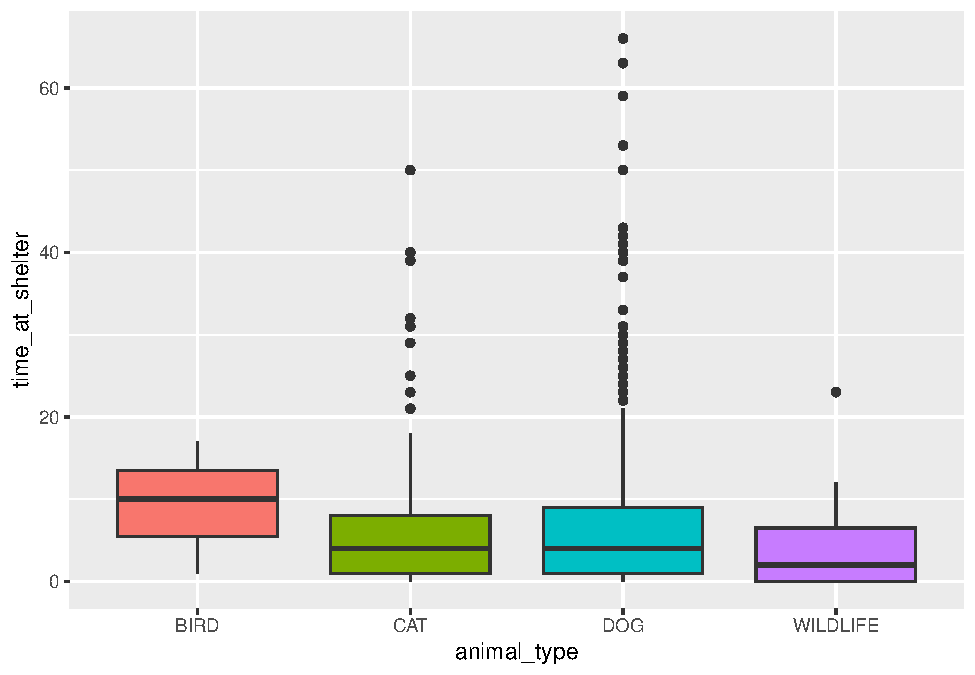
\includegraphics[width=0.68\linewidth]{Group_16_Project_files/figure-latex/unnamed-chunk-2-1} 

}

\caption{\label{fig:box} Figure 1:time\_at\_shelter by animal\_type}\label{fig:unnamed-chunk-2}
\end{figure}

Basically there is no difference of the days spent at the shelter
between being admitted and the final outcome for different animals in
2016 and 2017 ,which can be showed in Figure 2.

\begin{figure}[H]

{\centering 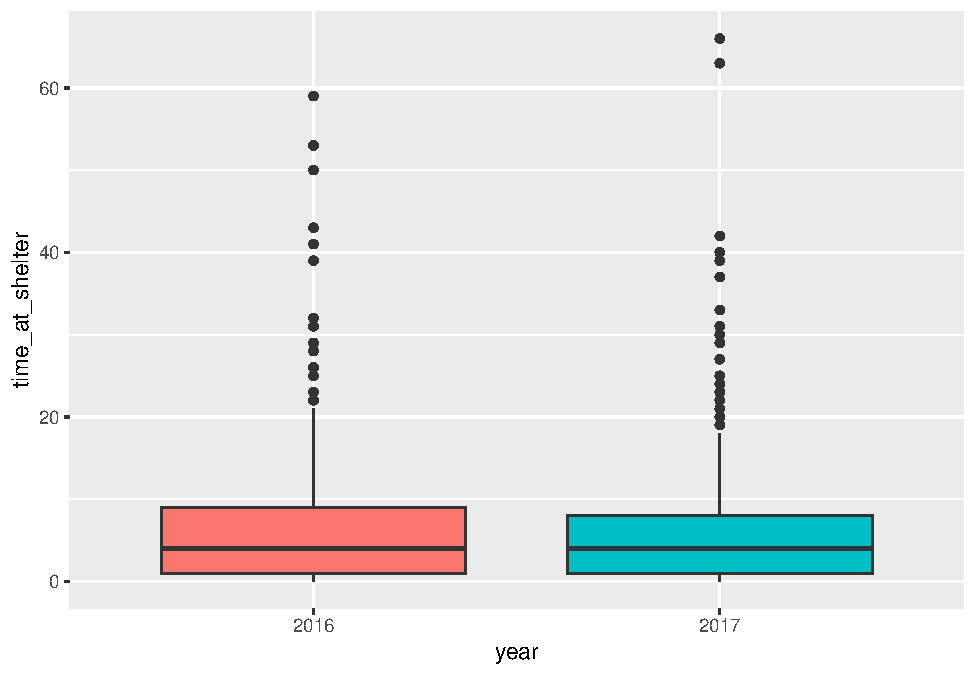
\includegraphics[width=0.68\linewidth]{Group_16_Project_files/figure-latex/unnamed-chunk-3-1} 

}

\caption{\label{fig:box} Figure 2:time\_at\_shelter by year}\label{fig:unnamed-chunk-3}
\end{figure}

From Figure 3,we can see that for different months,the days spent at the
shelter between being admitted and the final outcome for animals have
their own differences,but the median for 12 months all seem to be
similar.

\begin{figure}[H]

{\centering 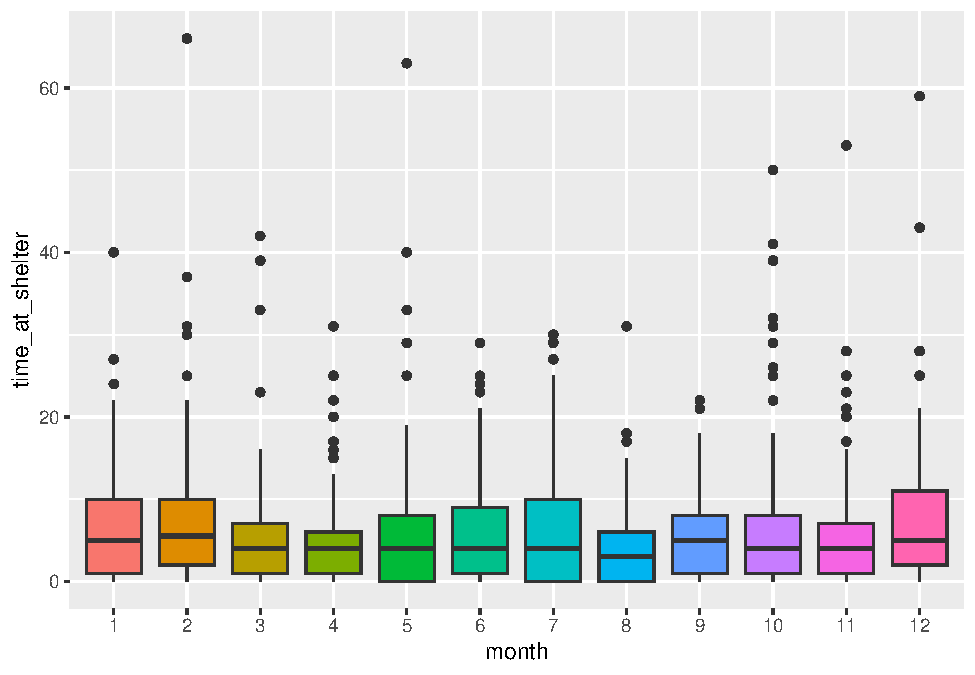
\includegraphics[width=0.68\linewidth]{Group_16_Project_files/figure-latex/unnamed-chunk-4-1} 

}

\caption{\label{fig:box} Figure 3:time\_at\_shelter by month}\label{fig:unnamed-chunk-4}
\end{figure}

As is showed in Figure 4, the confiscated animals stay longest time in
shelter before the outcome,and there are not too much difference for
owner surrendered and stray animals.

\begin{figure}[H]

{\centering 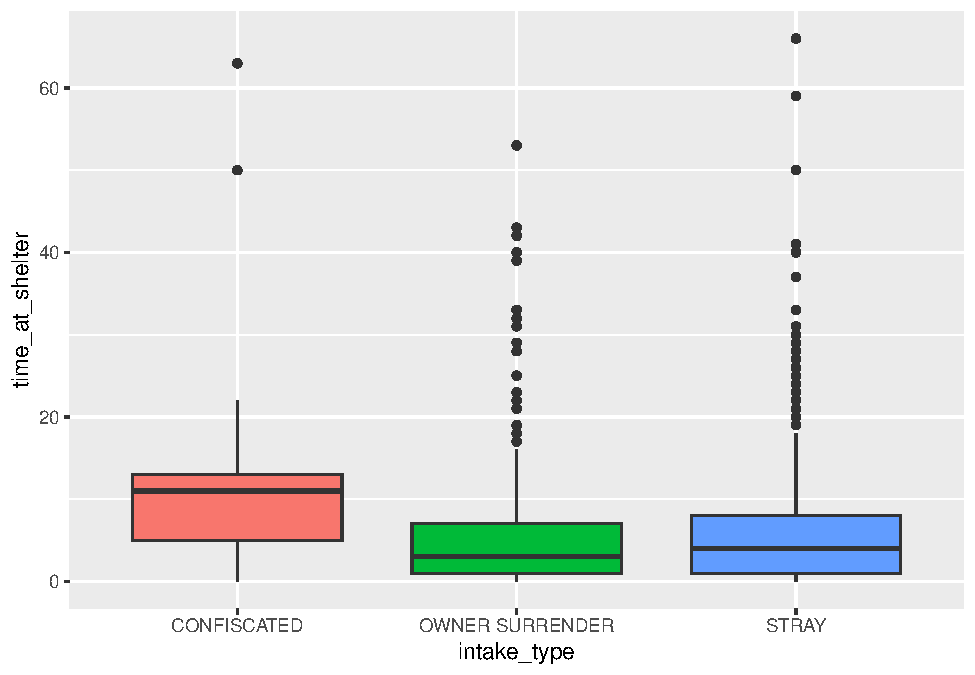
\includegraphics[width=0.68\linewidth]{Group_16_Project_files/figure-latex/unnamed-chunk-5-1} 

}

\caption{\label{fig:box} Figure 4:time\_at\_shelter by intake\_type}\label{fig:unnamed-chunk-5}
\end{figure}

In Figure 5,we can see that for the three types of chip status,the days
in shelter for animals with scanned chips have smallest median but
distribute more widely.

\begin{figure}[H]

{\centering 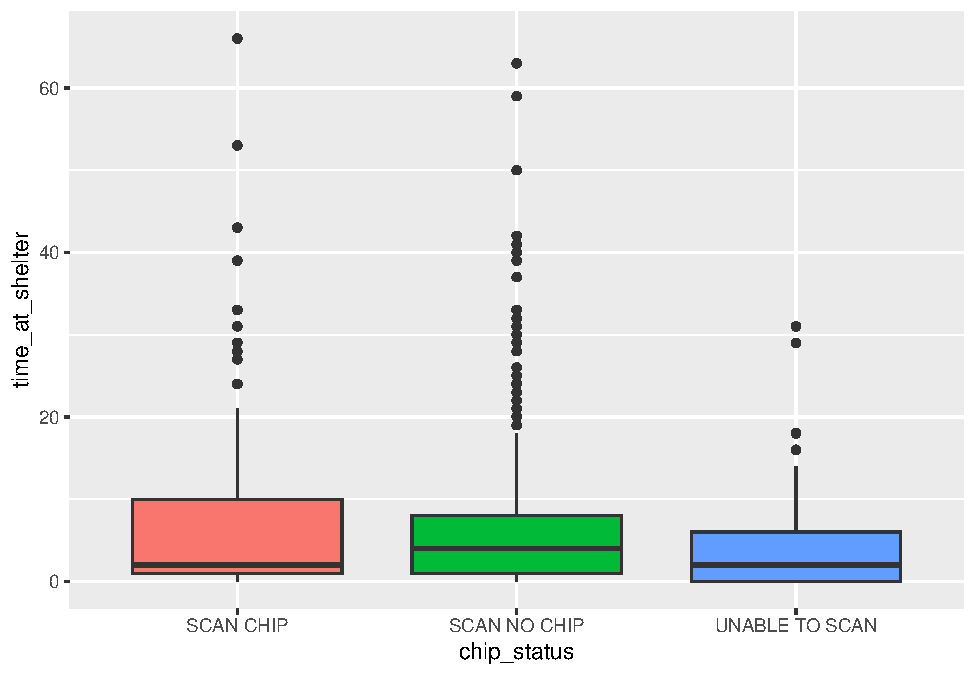
\includegraphics[width=0.68\linewidth]{Group_16_Project_files/figure-latex/unnamed-chunk-6-1} 

}

\caption{\label{fig:box} Figure 5:time\_at\_shelter by chip\_status}\label{fig:unnamed-chunk-6}
\end{figure}

\hypertarget{formal-data-analysis}{%
\section{Formal Data Analysis}\label{formal-data-analysis}}

After the initial graphical analysis of the relationship between the
variables, we will use the GLM model to further analyse the relationship
between the outcome variables (Time\_at\_Shelter)and the explanatory
variables(Animal\_type,Month,Year,Intake\_type,Chip\_Status), and the
model will be based on poisson GLM model, since the response variable is
the count of the number of days animal spent at the shelter, with link
function log.So,the model(1) will be like this: \[
\log(\mathrm{E}(y_i)) = \beta_0 + \beta_{1i} \mathrm{animal\_type_i} + \beta_{2j} \mathrm{month_j} + \beta_{3t} \mathrm{year_t} + \beta_{4p} \mathrm{intake\_type_p} + \beta_{5q} \mathrm{chip\_status_q}
\] where the value of \(\mathrm{animal\_type_i}\)
include:BIRD,CAT,DOG,WILDLIFE;the value of \(\mathrm{month_j}\)
include:1 to 12;the value of \(\mathrm{year_t}\) include:2016,2017;the
value of \(\mathrm{intake\_type_p}\)include:CONFISCATED,OWNER
SURRENDER,STRAY;the value of \(\mathrm{chip\_status_q}\) include:SCAN
CHIP,SCAN NO CHIP,UNABLE TO SCAN;and all the variables above are group
variables.

The outcome can be showed as follow,and we notice that the coefficient
of year factor cannot be defined.There are some reasons for that,firstly
the the explanatory variables month and year exist multicollinearity,and
there are also some missing month data in 2016,finally we can also find
that changes in year does not affect the outcome variable from Figure 2.

\begin{verbatim}

Call:
glm(formula = time_at_shelter ~ animal_type + month + year + 
    intake_type + chip_status, family = poisson(link = "log"), 
    data = df)

Deviance Residuals: 
    Min       1Q   Median       3Q      Max  
-4.9857  -2.6038  -0.7551   0.8060  12.7653  

Coefficients: (1 not defined because of singularities)
                           Estimate Std. Error z value Pr(>|z|)    
(Intercept)                 2.75306    0.19690  13.982  < 2e-16 ***
animal_typeCAT             -0.18315    0.19396  -0.944 0.345017    
animal_typeDOG             -0.23305    0.19251  -1.211 0.226055    
animal_typeWILDLIFE        -0.38615    0.22984  -1.680 0.092945 .  
month2                      0.14546    0.05533   2.629 0.008562 ** 
month3                     -0.25477    0.05692  -4.476 7.61e-06 ***
month4                     -0.28620    0.05657  -5.059 4.21e-07 ***
month5                     -0.11780    0.05181  -2.273 0.022996 *  
month6                     -0.08372    0.04991  -1.677 0.093482 .  
month7                     -0.14828    0.05051  -2.936 0.003327 ** 
month8                     -0.50955    0.05871  -8.679  < 2e-16 ***
month9                     -0.20499    0.05596  -3.663 0.000249 ***
month10                     0.05627    0.05167   1.089 0.276127    
month11                    -0.05734    0.05436  -1.055 0.291483    
month12                     0.16794    0.05157   3.257 0.001127 ** 
year2017                         NA         NA      NA       NA    
intake_typeOWNER SURRENDER -0.77494    0.04076 -19.012  < 2e-16 ***
intake_typeSTRAY           -0.58951    0.03765 -15.658  < 2e-16 ***
chip_statusSCAN NO CHIP    -0.01469    0.02805  -0.524 0.600525    
chip_statusUNABLE TO SCAN  -0.27589    0.06781  -4.068 4.73e-05 ***
---
Signif. codes:  0 '***' 0.001 '**' 0.01 '*' 0.05 '.' 0.1 ' ' 1

(Dispersion parameter for poisson family taken to be 1)

    Null deviance: 10551.2  on 1449  degrees of freedom
Residual deviance:  9957.4  on 1431  degrees of freedom
AIC: 14017

Number of Fisher Scoring iterations: 6
\end{verbatim}

So we can consider dropping the variable year and reconstruct the model
with the remaining four variables as explanatory variables,just like the
following model(2):

\[
\log(\mathrm{E}(y_i)) = \beta_0 + \beta_{1i} \mathrm{animal\_type_i} + \beta_{2j} \mathrm{month_j} + \beta_{3p} \mathrm{intake\_type_p} + \beta_{4q} \mathrm{chip\_status_q}
\] where all the values of these variables remain unchanged and they are
all group variables.

From the regression table below,we can see that the coefficients for
each of the explanatory variables were essentially negative, and in
terms of p-values, although some variables have p-values greater than
0.05 but given the correlated changes reflected in the box plots from
the previous preliminary analysis, all explanatory variables included in
the below regression model table are ultimately retained.

\begin{verbatim}

Call:
glm(formula = time_at_shelter ~ animal_type + month + intake_type + 
    chip_status, family = poisson(link = "log"), data = df)

Deviance Residuals: 
    Min       1Q   Median       3Q      Max  
-4.9857  -2.6038  -0.7551   0.8060  12.7653  

Coefficients:
                           Estimate Std. Error z value Pr(>|z|)    
(Intercept)                 2.75306    0.19690  13.982  < 2e-16 ***
animal_typeCAT             -0.18315    0.19396  -0.944 0.345017    
animal_typeDOG             -0.23305    0.19251  -1.211 0.226055    
animal_typeWILDLIFE        -0.38615    0.22984  -1.680 0.092945 .  
month2                      0.14546    0.05533   2.629 0.008562 ** 
month3                     -0.25477    0.05692  -4.476 7.61e-06 ***
month4                     -0.28620    0.05657  -5.059 4.21e-07 ***
month5                     -0.11780    0.05181  -2.273 0.022996 *  
month6                     -0.08372    0.04991  -1.677 0.093482 .  
month7                     -0.14828    0.05051  -2.936 0.003327 ** 
month8                     -0.50955    0.05871  -8.679  < 2e-16 ***
month9                     -0.20499    0.05596  -3.663 0.000249 ***
month10                     0.05627    0.05167   1.089 0.276127    
month11                    -0.05734    0.05436  -1.055 0.291483    
month12                     0.16794    0.05157   3.257 0.001127 ** 
intake_typeOWNER SURRENDER -0.77494    0.04076 -19.012  < 2e-16 ***
intake_typeSTRAY           -0.58951    0.03765 -15.658  < 2e-16 ***
chip_statusSCAN NO CHIP    -0.01469    0.02805  -0.524 0.600525    
chip_statusUNABLE TO SCAN  -0.27589    0.06781  -4.068 4.73e-05 ***
---
Signif. codes:  0 '***' 0.001 '**' 0.01 '*' 0.05 '.' 0.1 ' ' 1

(Dispersion parameter for poisson family taken to be 1)

    Null deviance: 10551.2  on 1449  degrees of freedom
Residual deviance:  9957.4  on 1431  degrees of freedom
AIC: 14017

Number of Fisher Scoring iterations: 6
\end{verbatim}

Finally,we transform the values in the model(2) into exponential
formFinally,we transform the values in the model(2) into exponential
form and plot the ratio of rates.In Figure 6, it can be seen that, from
the perspective of animal types, compared to birds, cats spent 0.83
times the number of days in the shelter, while dogs and other wild
animals spent 0.79 and 0.68 times the number of days, respectively. In
terms of the month the animal was admitted,compared to January, animals
admitted in December spend 1.46 times the number of days in the shelter,
which is the longest time, followed by animals admitted in February and
October, while animals admitted in all other months spend less number of
days in shelter than January, the smallest being animal admitted in
August, which is 0.6 times compared to animal admitted in January.In
terms of the reason for the animal being admitted,the confiscated
animals stay longest time in shelter,compared to them, the number of
days spend on shelter of animals with intake types of owner surrendered
and stray are of 0.46 and 0.55 times respectively.For chip
status,compared to the days spent in the shelter by animals with scan
chips, animals without scan chips and those unable to be scanned were
0.99 and 0.76 times, respectively.

\begin{figure}[H]

{\centering 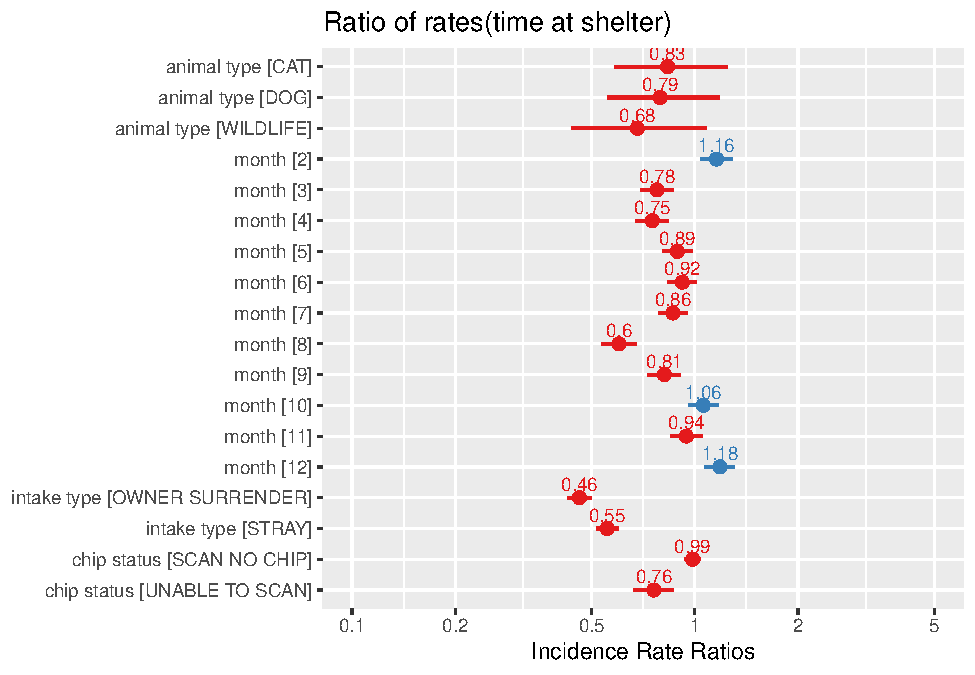
\includegraphics[width=0.68\linewidth]{Group_16_Project_files/figure-latex/unnamed-chunk-9-1} 

}

\caption{\label{fig:box} Figure 6:Ratio of rates(time at shelter)}\label{fig:unnamed-chunk-9}
\end{figure}

\hypertarget{conclusion}{%
\section{Conclusion}\label{conclusion}}

In summary, in order to find What factors influence the days of animals
spent at the shelter between being admitted and the final outcome
(Time\_at\_Shelter),we constructed the model based on poisson GLM model
with link function log to explore the relationship between the former
and the explanatory
variables(Animal\_type,Month,Year,Intake\_type,Chip\_Status), and
ultimately retains all variables except the year.Finally, by plotting
the ratio of rates, we also explored the quantitative relationship
between the variables within each type.

\end{document}
